\documentclass[../report.tex]{subfiles}

\begin{document}
\subsection{Đề bài} \cite{a-plus-b}
\begin{figure}[H]
\centering
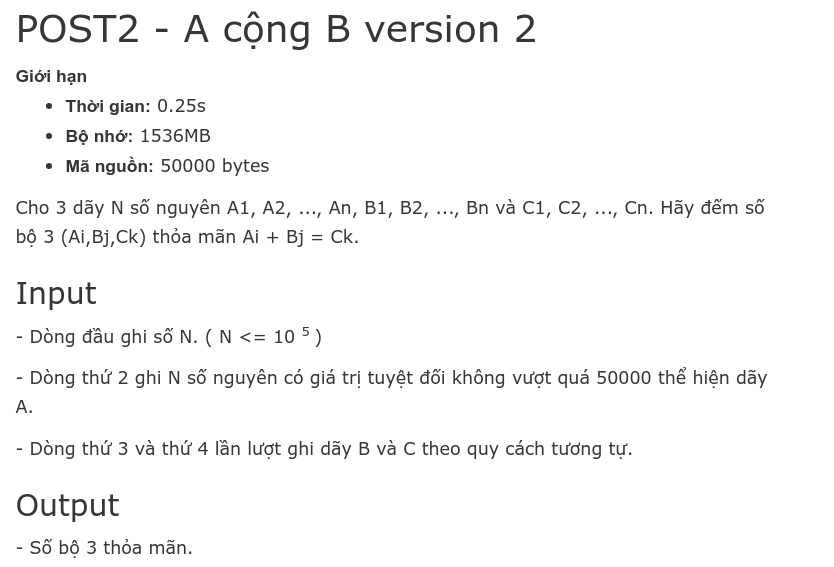
\includegraphics[width=\textwidth]{figures/a-plus-b.png}
\end{figure}

\subsection{Ý tưởng lời giải}
\begin{itemize}
    \item Mỗi giá trị của các dãy nằm trong khoảng từ
        $-50000$ đến $50000$ \\
        $\Rightarrow$ Có tổng cộng $100001$ giá trị. 
    \item Mỗi dãy A, B, C có thể đại diện bằng một vector (nguyên)
        $100001$ chiều. 
    \item Gọi U, V, W lần lượt là 3 vector đó.
    \item $\Rightarrow$ Số bộ 3 thỏa mãn là tổng: 

    \begin{align*}
        &N = 2^{\ceil{\log_2 (4n + 1)}} \\
        &R_k = \sum_{i = \max(-n, k - n) }^k U_i \times V_{k - i}
        \quad \quad \mathcal{O} (N \log N)\\
        &\sum_{k = -n}^n W_k R_k \quad\quad \mathcal{O}(n) 
    \end{align*}\\

    $i = \max(-n, k - n)$ do $k - i \le n$. 
    Công thức của $R_k$ giống công thức của phép nhân đa thức. 
    Trong đó $n = 50000$, $\Rightarrow 2n$ là bậc của đa thức tương 
    ứng với 3 vector U, V, W. Nên bậc của đa thức ứng với $R_k$ là 
    $4n$. 
\end{itemize}

\subsection{Code của thuật toán}
\begin{lstlisting}
    int N;
    std::cin >> N;

    for (int i = 0; i < N; i++) {
        int x; std::cin >> x;
        A[x + MAX] += 1;
    }

    for (int i = 0; i < N; i++) {
        int x; std::cin >> x;
        B[x + MAX] += 1;
    }

    for (int i = 0; i < N; i++) {
        int x; std::cin >> x;
        C[x + 2*MAX] += 1;
    }

    fft(A, MAX_BIT_COUNT);
    fft(B, MAX_BIT_COUNT);

    for (ll i = 0; i < FFT_MAX; i++)
        A[i] *= B[i];

    fft(A, MAX_BIT_COUNT, true);

    ll count = 0;
    for (int x = MAX; x <= 3 * MAX; x++)
        count += std::llround(A[x].real()) * C[x];

    std::cout << count << std::endl;
\end{lstlisting}
Trong đó, $MAX = 50000$, $MAX\_BIT\_COUNT = 18$ 
do $\ceil{\log_2 (4N + 1)} = 18$.
Ta thực hiện đọc vào các mảng A, B, C. 
Cứ mỗi giá trị x, ta tăng giá trị 
các mảng tại vị trí tương ứng lên 1. 
Mảng A, B phải cộng $MAX$ do giá trị nhỏ nhất của x là $-MAX$. 
Mảng C phải cộng $2 \times MAX$ do A, B đã cộng $MAX$ và ta lại muốn 
cộng các phần tử của A, B và so sánh với C. 
Thực hiện nhân nhân đa thức sử dụng FFT bằng gọi FFT cho mảng A, B,
nhân lần lượt từng phần tử của hai mảng với nhau, và thực hiện 
FFT ngược để ra được đa thức kết quả.

Ta tính tổng từ $x = MAX$ đến $3 MAX$ do các giá trị của mảng 
C chỉ có nghĩa tại các vị trí $x = MAX$ đến $3 MAX$.

\subsection{Bộ test và kết quả chạy} 
Test được chạy trên chương trình chấm tự xây dựng, trong đó các test 
bao gồm:
\begin{itemize}
    \item 5 test tay (kết quả được tính bằng tay). 
    \item 2 test có quy luật (tổng bẳng và tổng không bằng), 
        kích thước 1000 phần tử. 
    \item 2 test có quy luật (tổng bằng và tổng không bằng), 
        kích thước 100000 phần tử. 
    \item 12 test được sinh ngẫu nhiên bằng thuật toán đơn giản 
        (không dùng FFT) để kiểm tra tính đúng đắn, kích thước 1000 phần tử. 
    \item 5 test được sinh ngẫu nhiên bằng chương trình đích để 
        kiểm tra thời gian chạy, kích thước 100000 phần tử. 
\end{itemize}
Kết quả chạy test: 
\begin{figure}[H]
\centering
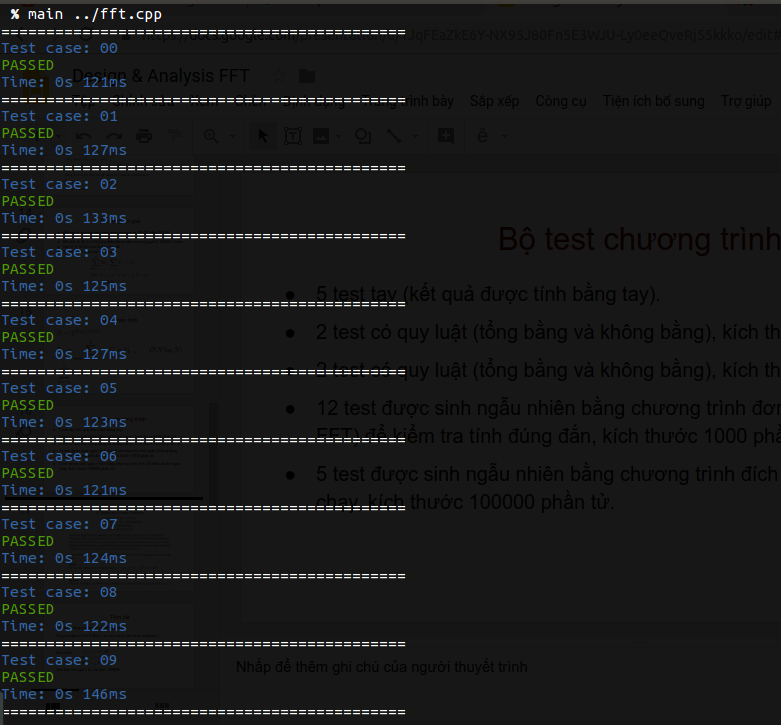
\includegraphics[width=\textwidth]{figures/test-a-plus-b-1.png}
\end{figure}

\begin{figure}[H]
\centering
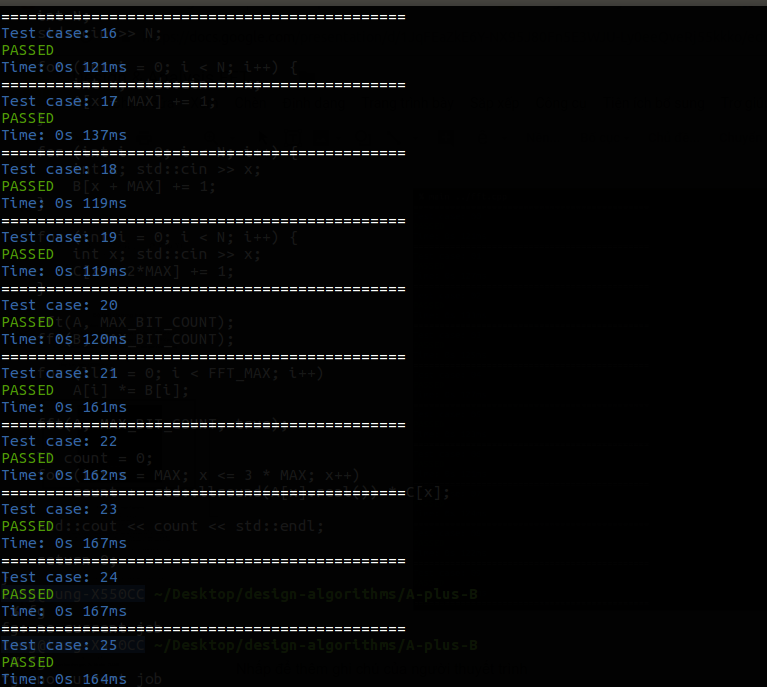
\includegraphics[width=\textwidth]{figures/test-a-plus-b-2.png}
\end{figure}

\subsection{Kết quả submit online}
\begin{figure}[H]
\centering
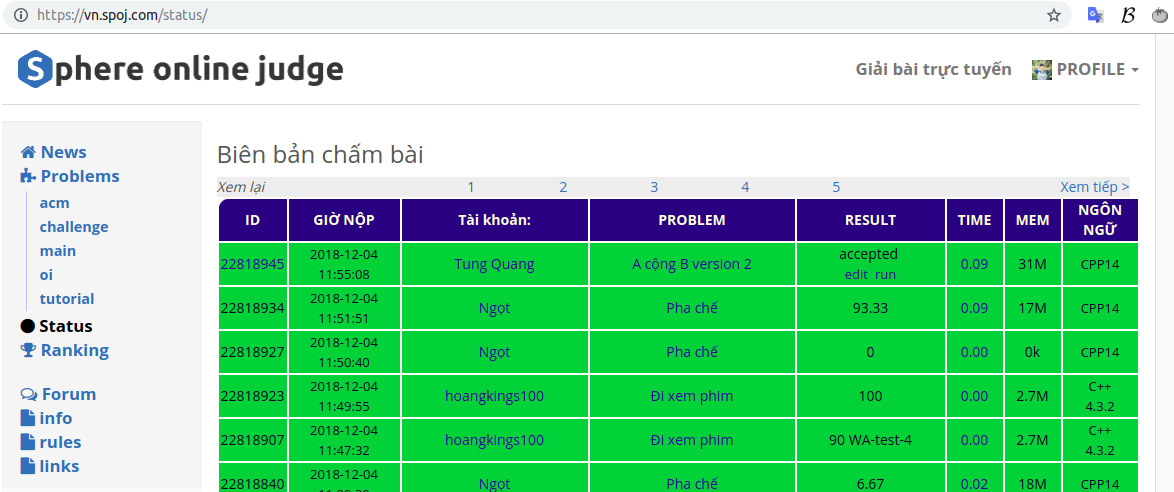
\includegraphics[width=\textwidth]{figures/submit-a-plus-b.png}
\end{figure}
\end{document}
